\subsection{Direction selective units in the optic tectum}

In total, we recorded 14371 units in the optic tectum of 3 zebrafish larvae (Figure \ref{fig:heatmap}). Our preprocessing pipeline extracted 129 units to be distinctly direction selective for either ccw or cw movement. Figure \ref{fig:heatmap} serves as an overview of the data set after it passed our preprocessing pipeline. The shade of the heatmap encodes the z-score of the respective ROI in the respective stimulus phase. It also illustrates the raw data, i.e. in the recorded temporal resolution instead of the means per phase. The bar on top illustrates single stimulus phases by a green and a red bar. The constrast levels for green and red where linearized for visualization purposes. Data in figure \ref{fig:heatmap} is visualized excluding the pauses of stimulation. Additionally, the previously randomized stimulation phases (motion direction and contrast levels) are now sorted. The left side shows the ccw moving stimulus phases and the right side the cw moving phases. On each side, all levels of green contrast are sorted by their combination with red contrast. The lowest row of the heatmap includes a subset of the units we excluded from our analysis. The second line from the bottom illustrates a subset of units that were considered to be 'active', i.e. showed auto-correlations that crossed our threshold. The two rows above show the complete dataset that passed the filtering steps and was included in the analysis. These rows nicely illustrate that the direction selective units we picked from the dataset using the regressor-correlation only show activity for their respective rotation direction. If we consider the chromatic stimulus levels, the same pattern appears in both populations: For stimuli with strong achromatic contrast, i.e. where red contrast is zero and green contrast increases (left sides of ccw and cw colums), the recorded calcium activity increases with increasing luminance contrast. If we consider the right side of the stimulus column for both populations, i.e. where red contrast is strongest and green contrast increases, we see the opposite pattern: While the luminance contrast is high, calcium activity is strong. But as the stimulus approaches isoluminance, i.e. chromatic contrast becomes the main driver of the response, calcium activity decreases.

\vspace{\baselineskip}

\begin{figure}[ht]
    \centering
    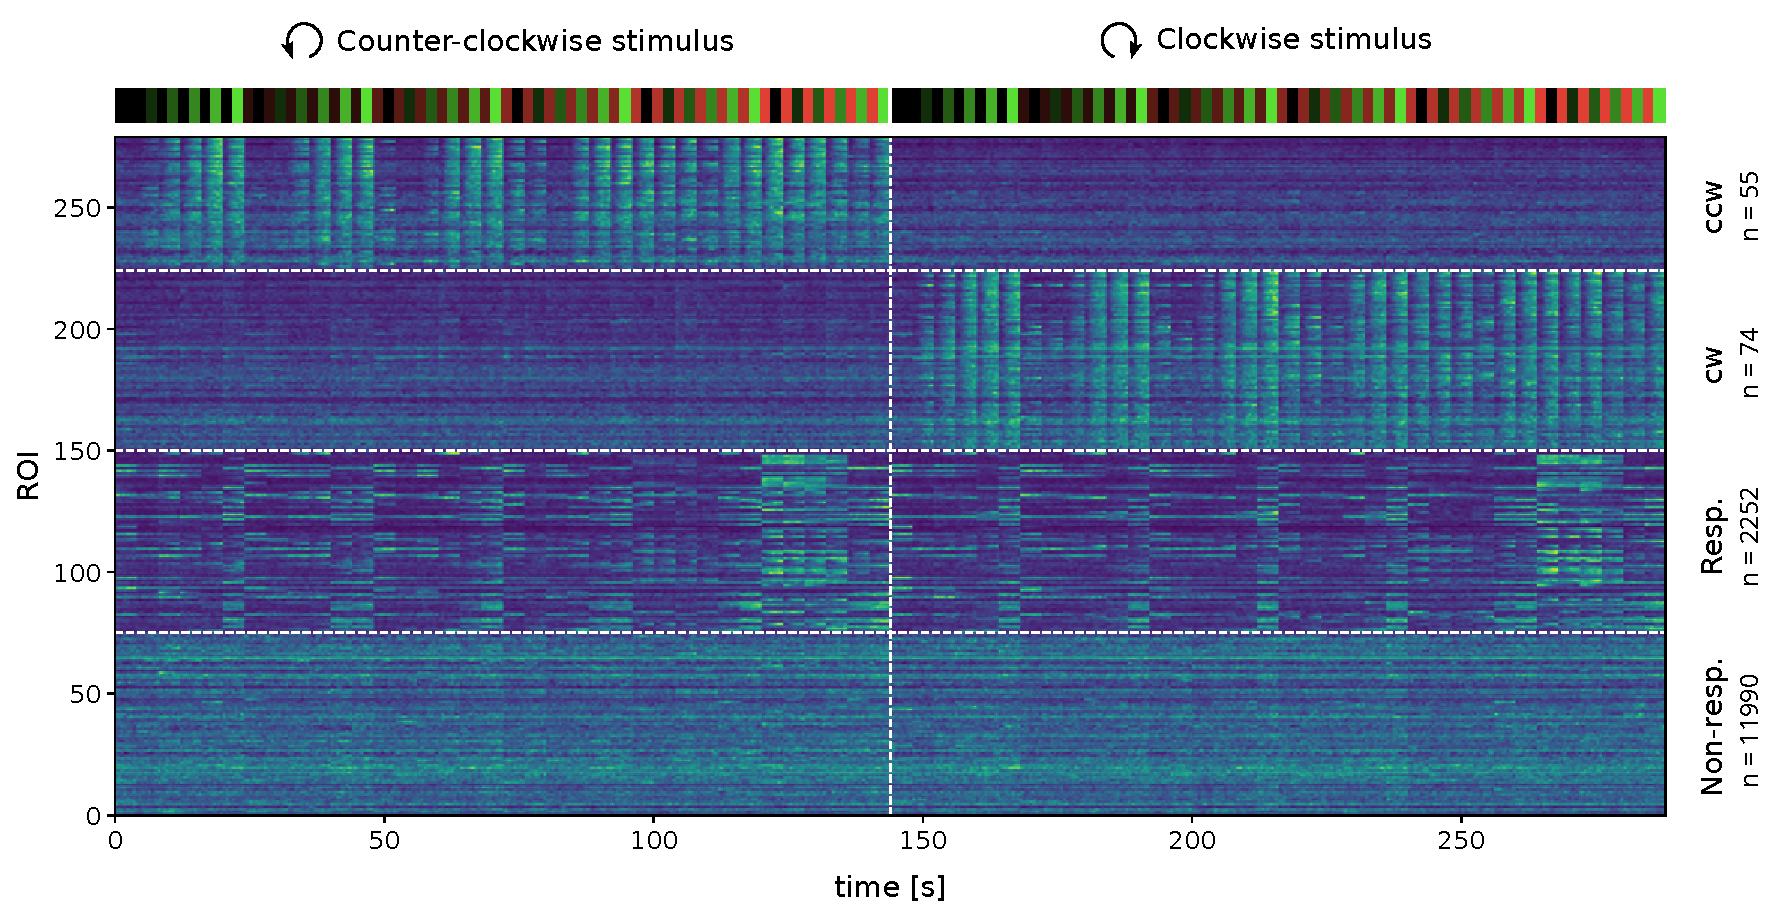
\includegraphics[width=\linewidth]{figures/testimg.pdf}
    \mycaption{Overview of selected ROIs}{ after they passed through our preprocessing pipeline. As opposed to our stimulus protocol, the data is sorted according to rotation direction and contrast levels. Data is plotted for just the fist of three stimulus repetitions. Units in the lowest category show now apparent pattern of activity in response to the stimulus. Units that are considered to be just responsive but not direction selective show a pattern that corresponds to the stimulus but does not change between the two rotation directions. Unit that where selected to be direction selective only show an activity pattern that corresponds to the stimulus in their respective rotation direction.}
    \label{fig:heatmap}
\end{figure}

In figure \ref{fig:calciumdata} we only included direction selective units and computed the mean and standard deviations for every stimulus phase across all individuals, ROIs, and repeats. The resulting data is plotted as a line plot for the combination of every single possible level of green contrast separately combined with all possible combinations of red contrast (figure \ref{fig:calciumdata}, (B) ). This is the same order that we chose to visualize the stimulus in figure \ref{fig:heatmap}. If the units we recorded did not respond to isoluminant chromatic contrasts, the line plots should show a trough where the red and green contrast is the same. This point is denoted by a dashed vertical line. For a green contrast level of 0 the minimum for both cw and ccw line plots is at 0. This is to be expected since motion is not supposed to be encodable if there is neither luminance nor chromatic cues that make it perceivable. For the green contrast levels of 0.1 and 0.18 however, the minima are both just right of the dashed vertical line. This indicates firstly, that a isoluminant chromatic contrast evokes the lowest response in direction selective units and secondly, that the green channel was perceived stronger than the red channel by the fish. The same pattern is observable for a green contrast of 0.32. For green contrast levels above that no trough is visible. 

\vspace{\baselineskip}

In figure \ref{fig:calciumdata}, (C) top, we visualized all possible stimulus combinations in the same way we visualized the mean z-scores from (B): All possible levels of green are plotted in the columns of the matrix and all possible levels of red contrast are plotted in the rows of the matrix. The luminance contrast increases strongest along the x- and y-dimension of the matrix, while the isoluminant, chromatic contrast increases along the diagonal of the matrix. Below that we then visualized the average z-scores that are already plotted in (B) in the same way. The resulting heat map shows an increase in the z-scores along the x- and y-axes, i.e. where luminance contrast increases. The diagonal, where the stimulus was assumed to be isoluminant and consisting of exclusively chromatic contrast, the heat map has a local minimum. This shows, that stimuli with more chromatic contrast than luminance contrasts resulted in lower activity in the direction selective neurons of the optic tectum. In addition, the heat map shows stronger activation along the x-axis (green contrast increase) compared to the y-axis (red contrast increase). This, in combination with the notion that the diagonal of inactivity is shifted towards the red channel, supports the assumption that the green channel was perceived stronger by the fish.


\begin{figure}[ht]
    \centering
    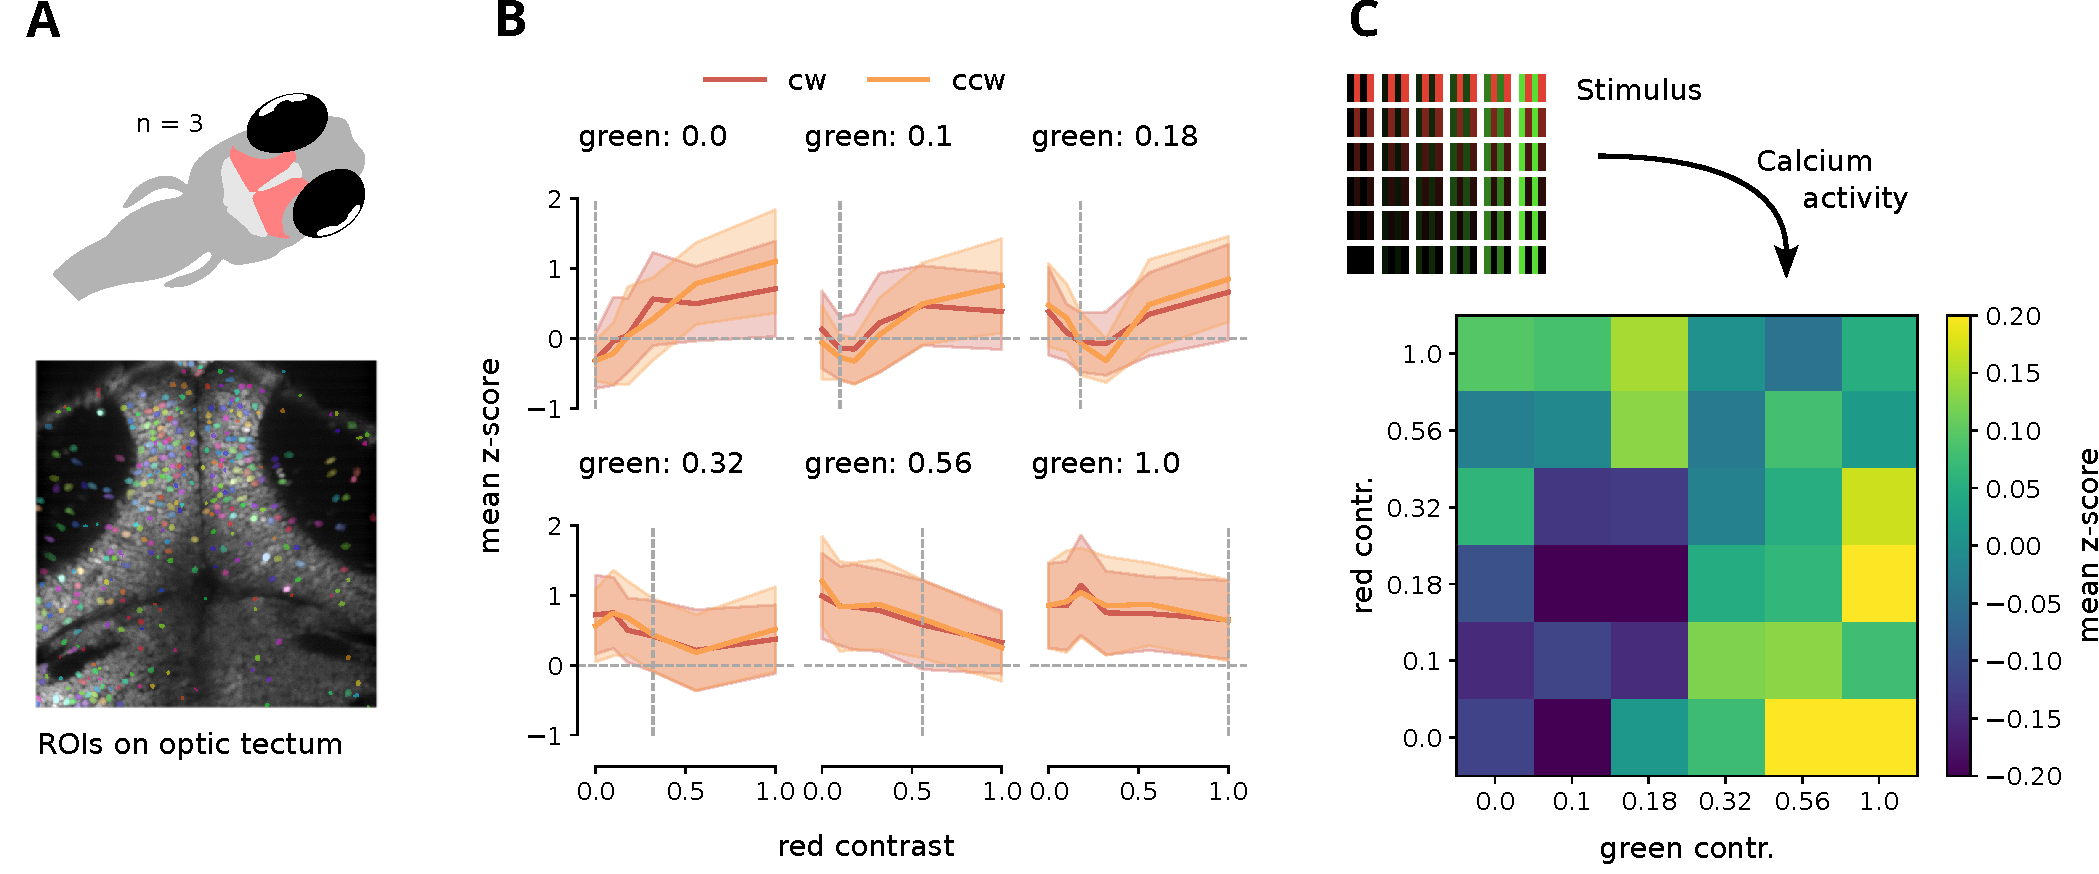
\includegraphics[width=\linewidth]{figures/contrast_curves_ca.pdf}
    \mycaption{Calcium activity for different contrast levels.}{(A) Location of the optic tectum in the brain of a zebrafish embryo. The lower figure illustrates the regions of interest in the optic tectum for which the activity was measured. (B) The mean z-score in all active units for ccw (orange) and cw (red) direction selective units. Each subplot shows the mean and standard deviation for one distinct level of green contrast in comparison to all possible combination of red contrast for this respective green level. The dashed vertical line denotes the value on the x-axis for which only color contrast was expected to drive a response. Thus we expect troughs in activity at the positions of the dashed line. (C) Shows the different levels of the stimulus contrast illustrated in a matrix where red contrast decreases in each row and green contrast increases in each column. The heat map below illustrates the mean z-score pooled for both rotation directions organized in the same way as the stimulus matrix. If given the assumption that red and green contrast was perceived equally and that color contrast alone does not drive the activity of motion direction selective units, we expected diagonal with low z-scores.}
    \label{fig:calciumdata}
\end{figure}

\subsection{Optokinetic response}

Figure \ref{fig:behavdata} shows the recorded eye velocities in a similar manner as the calcium data visualized in figure \ref{fig:calciumdata}. Panel (B) shows the mean eye velocities in all stimulus phases computed across both subjects and all stimulus repeats. Each subplot illustrates a single level of green contrast in combination with all possible levels of red contrast. If the driver of the observed behavior was luminance more than chromaticity, we should again see a trough in the mean eye velocity where the levels of green and red contrasts were the same, i.e. at the dashed vertical lines. As in figure \ref{fig:calciumdata}, the trough approximately follows the dashed vertical line through the subplots. Again, the same pattern is observable in panel C of figure \ref{fig:behavdata}. The diagonal includes the lowest mean eye velocities, suggesting that the behavioral response was mainly driven by the luminance, instead of chromaticity. As in figure \ref{fig:calciumdata} (C), the diagonal is slightly shifted upwards. This further strengthens our assumption, that the green channel was perceived with a higher intensity. 

\begin{figure}[H]
    \centering
    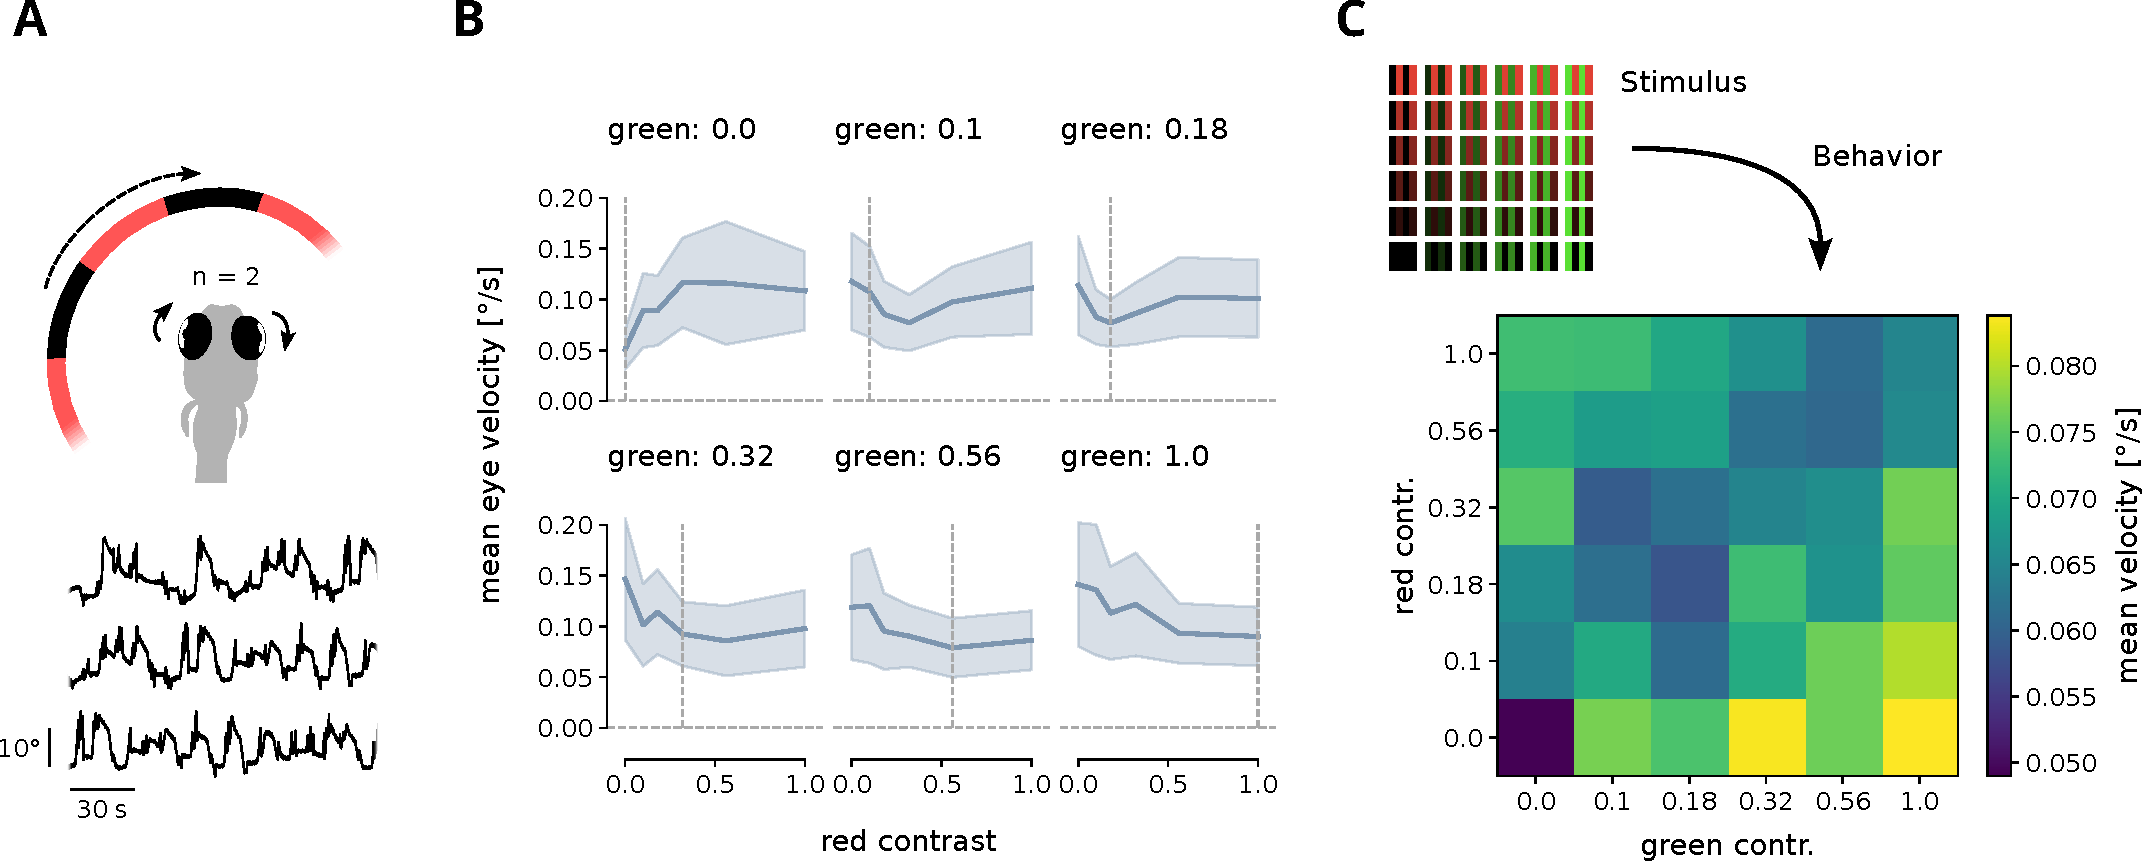
\includegraphics[width=\linewidth]{figures/contrast_curves_behav_test.pdf}
    \mycaption{Behavioral responses to different contrast levels.}{(A) Illustration of stimulus presentation and saccadic measurements to quantify the optokinetic response. (B) Mean and standard deviation of eye velocity for every level of green contrast (each subplot) as a function of all possible corresponding red contrast levels. The dashed vertical line illustrates the point in which, given that contrasts are perceived equally, only chromatic contrast should govern the behavioral response. If fish did not respond to exclusively color contrasts, the trough of the mean line should follow this point on the x-axis. (C) Stimulus and behavioral results quantified in the mean eye velocity are plotted in the same way as described in figure \ref{fig:calciumdata}. If the chromatic contrast did not contribute to the behavioral response, we would expect a diagonal of decreased eye velocity.}
    \label{fig:behavdata}
\end{figure}